\documentclass[12pt]{article}
\usepackage{amssymb}
\usepackage{enumerate}
\usepackage{commath}
\usepackage{fontspec} 
\usepackage{xeCJK}
\usepackage[left=2cm,right=2cm,top=2cm,bottom=2cm]{geometry}
\usepackage{amsmath}
\usepackage{listings}
\usepackage{graphicx}
\parindent=0pt
\setCJKmainfont{標楷體} 
\XeTeXlinebreaklocale "zh"
\XeTeXlinebreakskip = 0pt plus 1pt
\title{數值分析Team5 Homwork3}
\author{盧勁綸\and 張毓軒\and 李奇軒\and 王宥鈞}
\date{}


\begin{document}
\maketitle

[Theoretical problems] 修改1.(d)(e)
\begin{enumerate}
    \item
        \begin{enumerate}
            \item %1(a) 
            \begin{eqnarray*}
                T_0=\cos(0*\cos^{-1}x)=1 \\
                T_1=\cos(1*\cos^{-1}x)=x 
            \end{eqnarray*} 
            Let $T_{n-1}=\cos((n-1)*\cos^{-1}x)$
            \begin{eqnarray*}
                2x*T_{n-1}&=&2\cos(\frac{2}{2}*\cos^{-1}x)*\cos(\frac{2n-2}{2}*\cos^{-1}x)\\
                &=&2\cos(\frac{n-(n-2)}{2}*\cos^{-1}x)*\cos(\frac{n+(n-2)}{2}*\cos^{-1}x)\\
                &=&\cos(n*\cos^{-1}x)+\cos((n-2)*\cos^{-1}x)\\
                &=&T_n+T_{n-2}\\
            \end{eqnarray*}
            
            \item %1(b)
            For $x\in[-1,1],\ k\in\  \mathbb{Z} $
            \begin{eqnarray*}
            \cos(n*\cos^{-1}x_k)&=&0\\
            n*\cos^{-1}x_k&=&\cos^{-1}0\ \ =\ \ \frac{2k-1}{2}\pi\\
            \cos^{-1}x_k&=&\frac{2k-1}{2n}\pi\\
            x_k&=&\cos(\frac{2k-1}{2n})\pi
            \end{eqnarray*}
            For $k=1,2,\cdots,n$ , we have n zeros.
            
            \item %1(c)
            \begin{eqnarray*}
            (T_n)'=\cos(n\cos^{-1}\tilde{x}_k)'&=&0\\
            \sin(n\cos^{-1}\tilde{x}_k)(\frac{n}{\sqrt{1-\tilde{x}_k^2}})&=&0\\
            \sin(n\cos^{-1}\tilde{x}_k)&=&0\\
            n\cos^{-1}\tilde{x}_k&=&k\pi\ ,\ \ k\in\ \mathbb{Z}\\
            \cos^{-1}\tilde{x}_k&=&\frac{k\pi}{n}\\
            \tilde{x}_k&=&\cos\frac{k\pi}{n}\\            
            \end{eqnarray*}
            For $k=0,1,2,\cdots,n$ , we have n+1 zeros.
            \begin{eqnarray*}
                T_n(\tilde{x}_k)&=&\cos(n\cos^{-1}(\cos\frac{k\pi}{n}))\\
                &=&\cos(n*\frac{k\pi}{n})\\
                &=&\cos(k\pi)\\
                &=&(-1)^k
            \end{eqnarray*}
            
            \item %1(d)
            Since $\max\abs{T_n(x)}=1$ , the problem can be reduce as
            \begin{equation*}
                \frac{1}{2^{n-1}}\le\max_{-1\le x\le1}\abs{p(x)}\\
            \end{equation*}
            By the hint , assume $\exists\  p \in P_n$
            \begin{equation*}
            \max_{x\in[-1,1]}\abs{p(x)} < \frac{1}{2^{n-1}}\\
            \end{equation*}
            Consider function $r=\frac{T_n}{2^{n-1}}-p$ , $p\not=\frac{T_n}{2^{n-1}}$ , and deg $r\le n-1$\\
            By Fundamental Theory of Algebra , \# roots of r $\le n-1$\\
            But $\abs{p(x)}\le\norm{\frac{T_n}{2^{n-1}}}_\infty\ ,\ \forall x\in [-1,1]$\\
            \# of the roots shouldn't be less than n $\Rightarrow$ \# roots of r $\ge n \rightarrow\leftarrow$\\
            therefore , $\forall p \in P_n$\\
            \begin{equation*}
                \max_{x\in[-1,1]}\frac{\abs{T_n}}{2^{n-1}}\le\max_{-1\le x\le1}\abs{p(x)}\\
            \end{equation*}
            
            \item %1(e)
            Since $(x-x_0)\cdots(x-x_n)\in P_{n+1}$\\
            Choose $\tilde{x}_k=\cos(\frac{2k+1}{2(n+1)}\pi)\ ,\ k=0,\cdots,n$\\ 
            to minimize the maximum of $(x-x_0)\cdots(x-x_n)$\\
            by (d) we get\\
            \begin{equation*}
                \frac{1}{2^n}=\max_{-1\le x\le 1}\abs{(x-\tilde{x}_1)\cdots(x-\tilde{x}_n)}\le \max_{-1\le x\le 1}\abs{(x-x_1)\cdots(x-x_n)}
            \end{equation*}
           Since $f^{(n+1)}$ is continuous, by extreme value theorem, there exist $X= \max |f(x)|,~\text{where}~ x \in [-1,1]$. Therefore, the maximal error should be
           \begin{align*}
           \Longrightarrow &\max_{x\in(-1,1)}\abs{f(x)-p(x)} \\\\
           =&\max_{x\in(-1,1)}\abs{\dfrac{f(\xi(x))}{(n+1)!}}\cdot\abs{(x-\tilde{x_1})(x-\tilde{x_2})\cdots(x-\tilde{x_n})}\\\\
           \leq &\abs{\dfrac{M}{(n+1)!}}\max_{x\in(-1,1)}\abs{(x-x_1)\cdots (x-x_n)}
           \end{align*}
           where $x_i$ are randomly picked in (-1,1) satisfy $-1=x_0<x_1<\cdots<x_n=1,~\forall~i$
        \end{enumerate}
\end{enumerate}
\newpage
[Numerical Problems]修改1.和3.
\begin{enumerate}
    \item
        \begin{enumerate}
            \item %1(a)
                \lstset{language=Matlab,showstringspaces=false}
                \section*{for $n_1 = 11$}
                \lstinputlisting[frame=single,numbers = left]{interpolation11.m}
                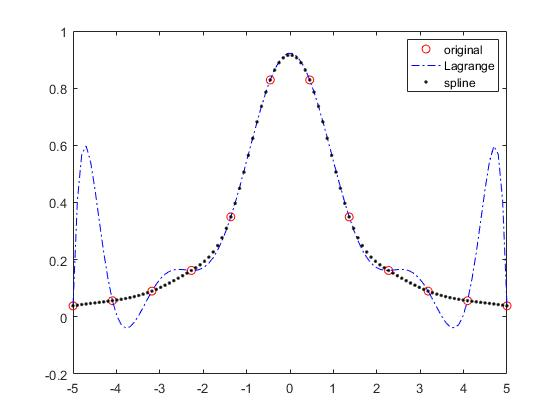
\includegraphics[width=5in]{11.jpg}\\
                \section*{for $n_2 = 21$}
                \lstinputlisting[frame=single,numbers = left]{interpolation21.m}
                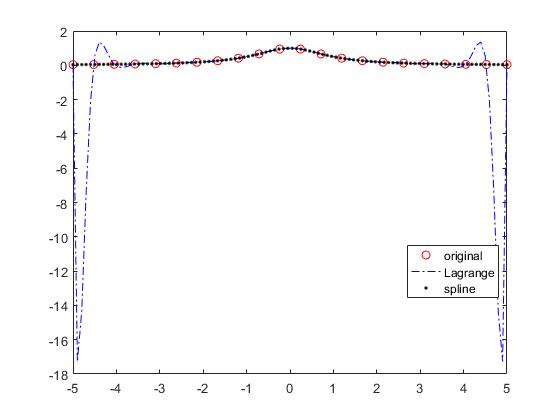
\includegraphics[width=5in]{21.jpg}\\
            
            \item %1(b)
            As $n \to \infty$ , the biggest error in the interval will also approximate infinity .  
            
            \item %1(c)
                \section*{for $n_1 = 11$}
                \lstinputlisting[frame=single,numbers = left]{cinterpolation11.m}
                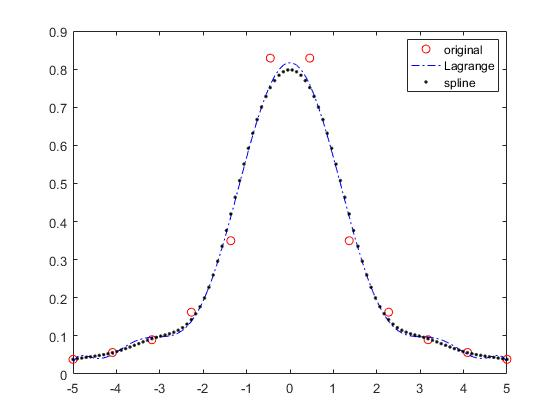
\includegraphics[width=5in]{c11.jpg}\\
                \section*{for $n_2 = 21$}
                \lstinputlisting[frame=single,numbers = left]{cinterpolation21.m}
                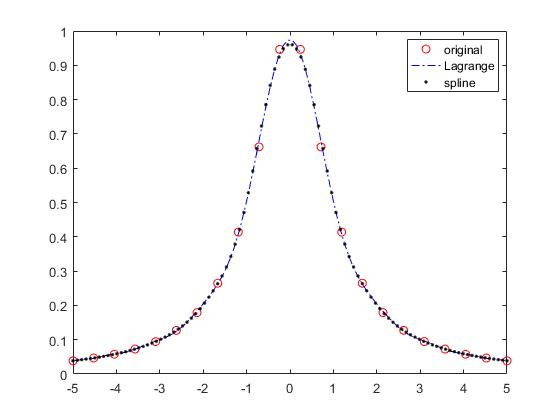
\includegraphics[width=5in]{c21.jpg}\\
        \end{enumerate}
\end{enumerate}
\end{document}
